\subsubsection{Mechanics} \label{sec:mechanics}
% 3D Printed Frame
To house the components, a 3D-printed housing was designed. It features a modular design, allowing for an iterative design process
where different components of the system can be worked on independently. It also allows for easy replacement of components
should the design prove to be inadequate. The housing was designed in FreeCAD\cite{freecad}, a free and open-source parametric CAD software. \\
The parametric design allows for easy modification of the design should changes need to be made -
with good design practices, large systematic changes can be made by simply modifying a few numerical parameters.
The design was then printed using a 3D printer, a heavily modified Voxelab Aquila C2. 

All parts are printed in PLA (Polylactic Acid), a biodegradable thermoplastic that is commonly used in 3D printing\cite{Ranakoti2022}. The design
at this stage does not require any special properties from the material, so PLA is sufficient. The biodegradable properties of PLA
also align with the ethical considerations of the project, as discussed in Section \ref{sec:els} (Ethical, Legal, and Safety Plan). \\

For this stage of the project, three major components for the housing were designed:

\noindent
\textbf{PSU Housing} \\
The PSU housing contains the power supply and ensures that all high-voltage components are safely enclosed.
It also houses the power switch, the power socket and the terminals. As step-down converters are required for the Pi and LED Ring,
the PSU housing also contains mounting points for the step-down converters, as well as a mounting plate to ensure that the step-down converters
are mounted flat to the PSU housing.

\noindent
\textbf{Camera Housing}
\label{sec:camerahousing} \\
The camera housing contains the camera and the LED Ring. It also contains the mounting points for the camera and LED Ring.
The camera housing will also mount an acrylic plate above the camera, so components can be placed on the plate and be imaged by the camera. \\
From bottom to top in Figure \ref{fig:camerahousing}, are the bottom casing, LED Ring mount, camera mount, light diffuser, middle casing and
top casing. \\

\noindent
\textbf{LCD Display Housing}
\label{sec:lcdhousing} \\
The LCD housing contains the LCD and the Raspberry Pi. As the 7" DFRobot LCD has a Raspberry Pi 4 mount on its back,
an explicit mount for the Pi is not required. The mount will position the LCD at an angle, so it can be viewed from above. The LCD
simply slides into the mount, allowing for easy removal and also contains mounting points to secure the LCD to the camera housing. \\
The LCD housing is split into two parts; the LCD cover, where the LCD slides into, and a base plate, which mounts to the camera housing.
The LCD cover is then mounted onto the base plate, securing the LCD in place.

The components are secured using brass M3 heat-set inserts and M3 screws. The heat-set inserts are inserted into the 3D-printed parts using a soldering iron,
and the components are then screwed into the inserts. This allows for easy removal of components should changes need to be made to the design, following
the modular design principle.

The design of the system at this stage is shown in the Appendix in Figure \ref{app:freecad}.
\begin{figure*}
    \begin{minipage}[t]{0.49\textwidth}
      \centering
      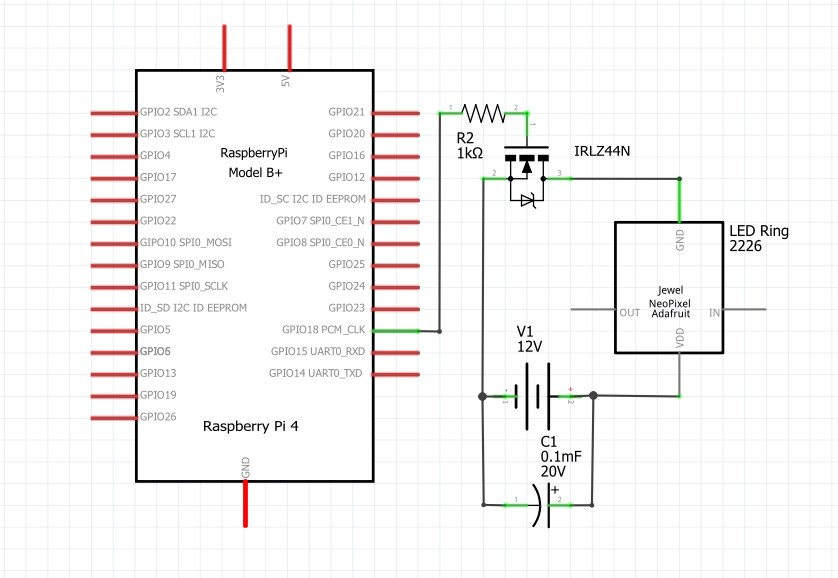
\includegraphics[width=\textwidth,height=5cm, keepaspectratio]{imgs/diagrams/wiring.jpg}
      \caption{Wiring Schematic for MOSFET, made with Fritzing\cite{fritzing}}
      \label{fig:wiringschematic}
    \end{minipage}
    \hfill
    \begin{minipage}[t]{0.49\textwidth}
        \centering
        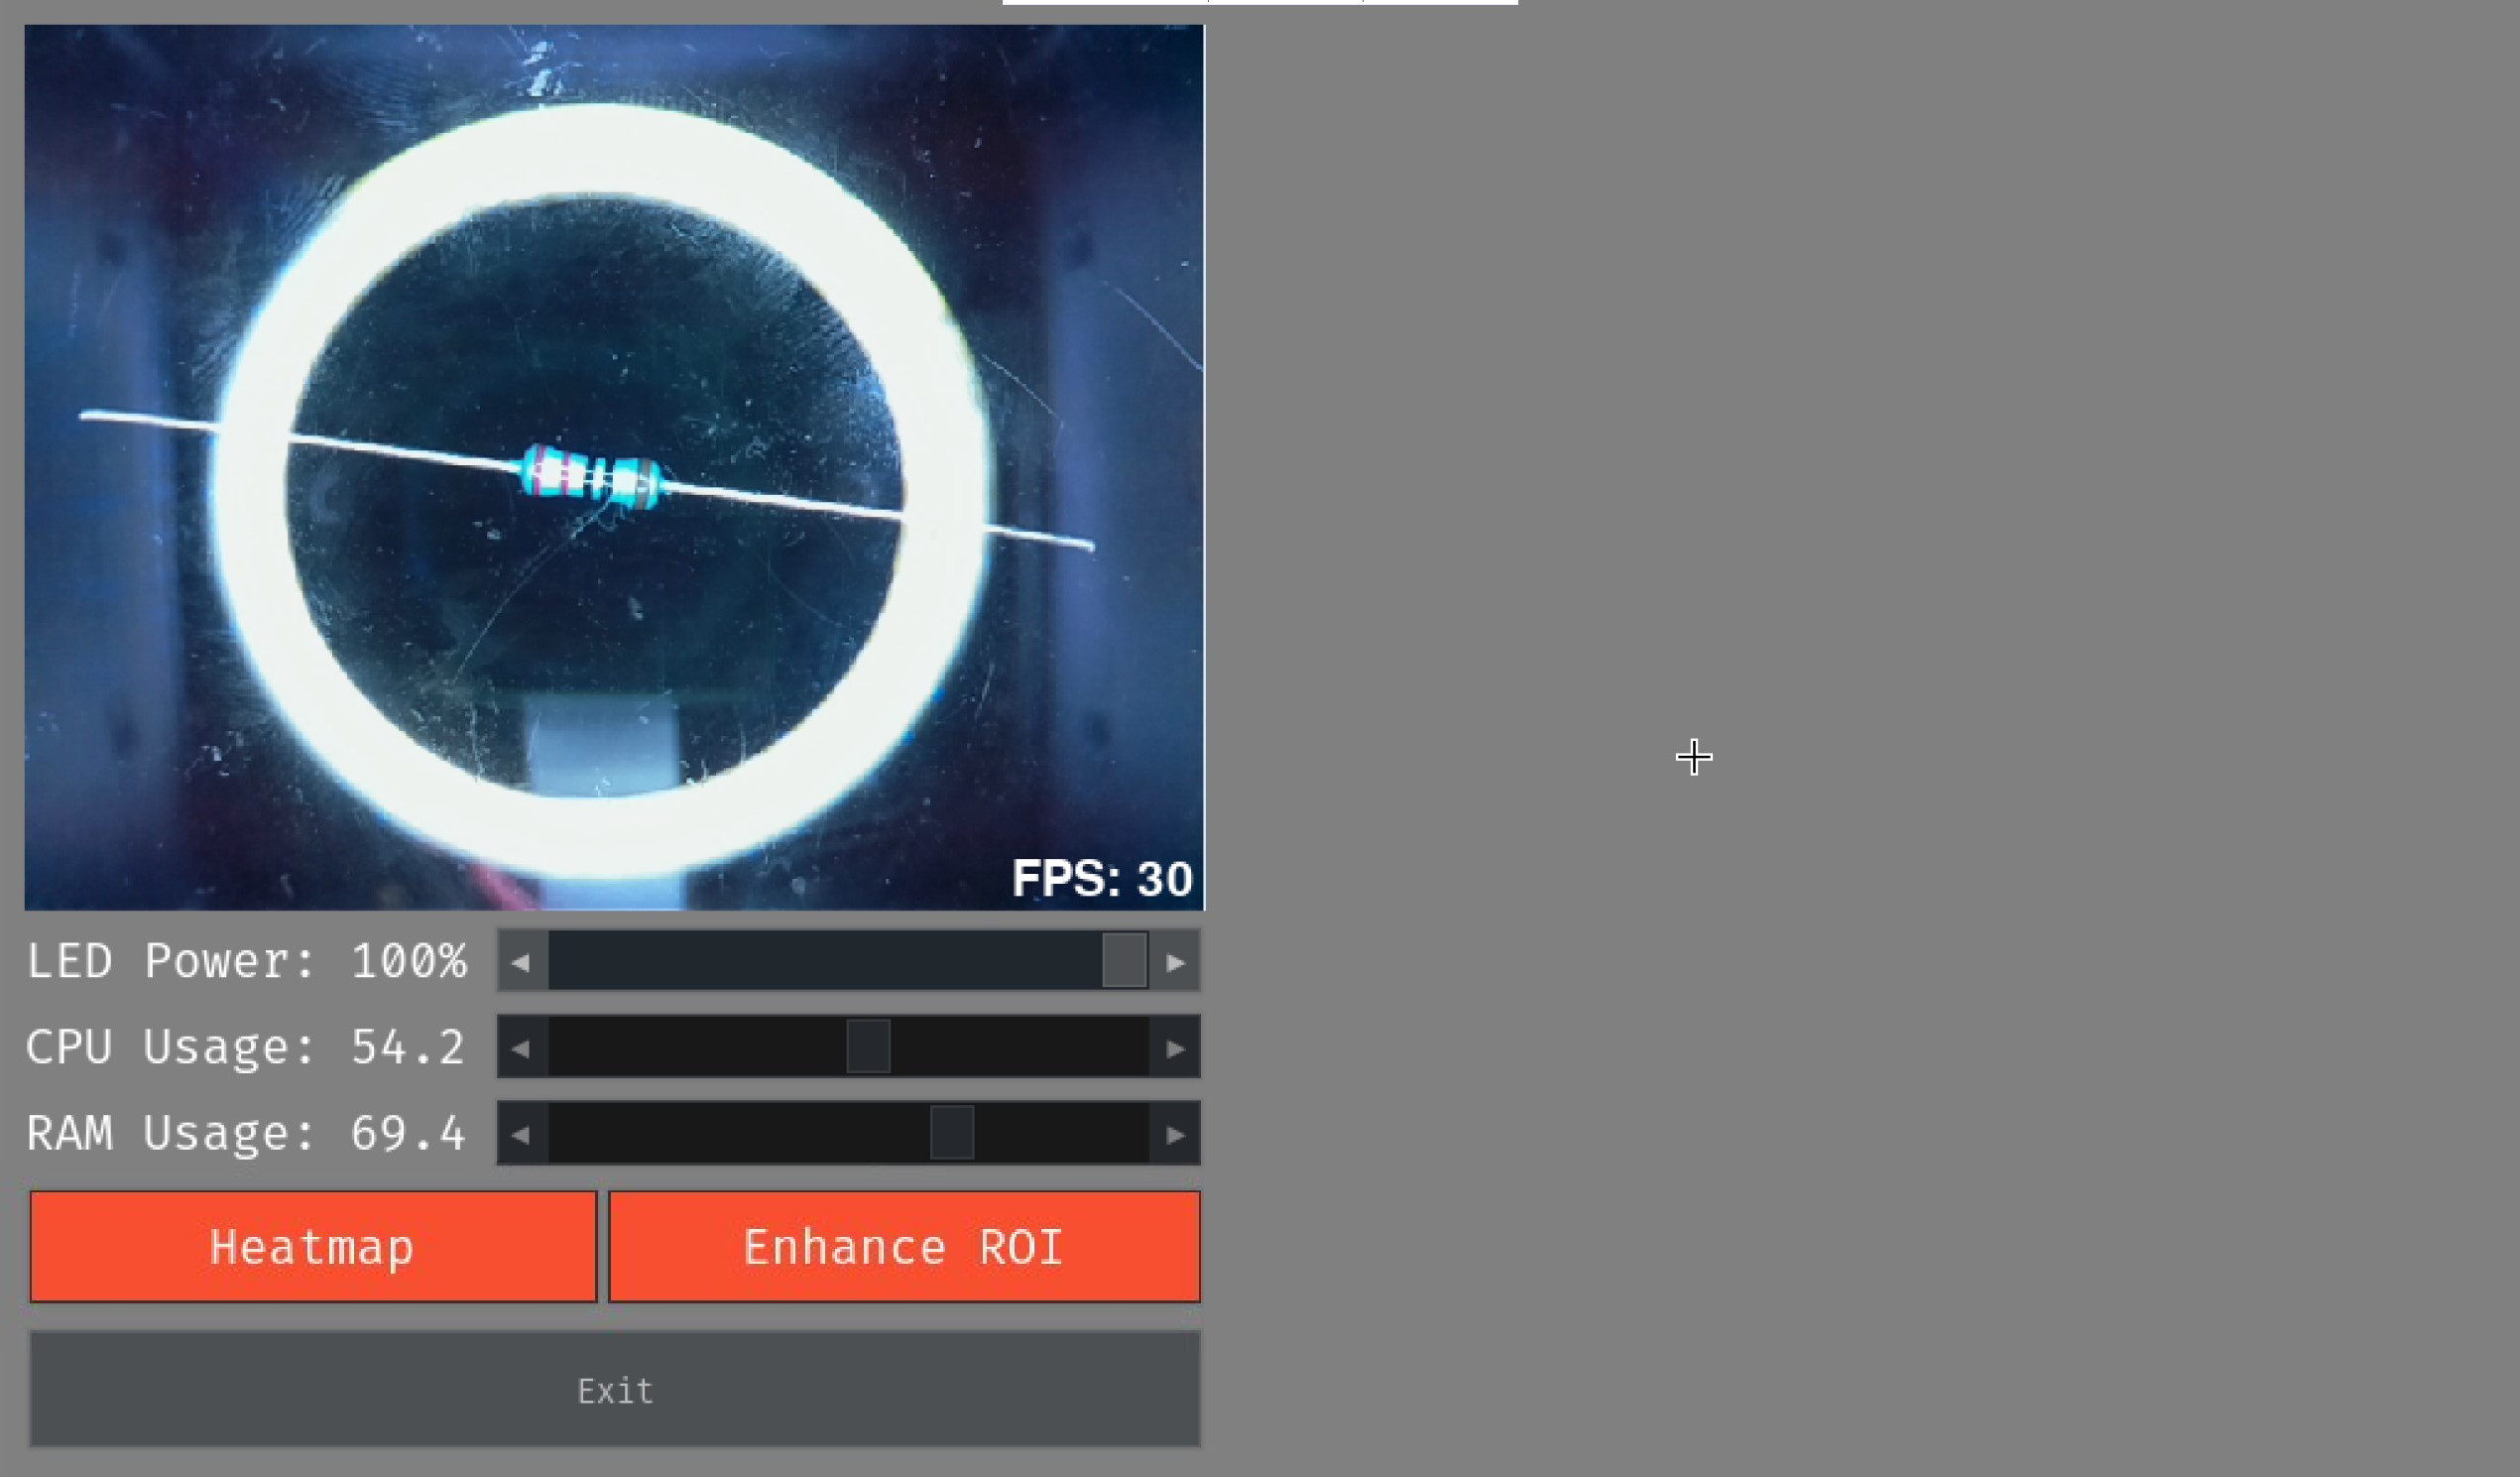
\includegraphics[width=\textwidth,height=5cm, keepaspectratio]{imgs/software/realvnc.jpg}
        \caption{Main UI, captured using RealVNC\cite{realvnc}}
        \label{fig:mainui}
    \end{minipage}
  \end{figure*}
  